\section{Experiments}

\subsection{Experimental Settings}
\paragraph{Datasets}
%Describe the two datasets.
We evaluate our approach on two datasets, including one English datasets and one Chinese dataset.

The English dataset, DBpedia dataset, is the one generated by \cite{chen2014encoding}, by mapping the triples in DBpedia \cite{bizer2009dbpedia} to the sentences in New York Time corpus. It has 51 different relations, includes about 50,000 entity tuples, 134,000 sentences for training and 30,000 entity tuples, 53,000 sentences for testing.

The Chinese dataset, HudongBaiKe dataset, is also generated by \cite{chen2014encoding}, they derive knowledge facts and construct a Chinese KB from the Infoboxes of HudongBaiKe, one of the largest Chinese online encyclopedias. They collect four national economic newspapers in 2009 as their corpus. 28 different relations are mapped to the corpus and this results in 60,000 entity tuples, 120,000 sentences for training and 40,000 tuples, 83,000 sentences for testing.

\paragraph{Hyperparameters}
%Describe the hyper parameters.
We use a grid search to determine the optimal parameters. For the Base Model, the CNN window size is 3, the Sentence embedding size is 256, position dimension is 5, batch size is 50, and the word embedding size is 50 for DBpedia dataset, 300 for Chinese dataset. The semantic loss rate for type constraints is 0.001 for DBpedia dataset, 0.005 for Chinese dataset, the semantic loss rate for Cardinality both for DBpedia and Chinese is 0.0005.
For the simplified semantic loss, the semantic loss rate for type constraints is 0.1 for DBpedia dataset, 0.1 for Chinese dataset, the semantic loss rate for Cardinality both for DBpedia is 0.0005 and for Chinese is 0.0005.

\iffalse
\begin{table}[!t]  
	\centering  
	\scriptsize  
	\caption{Parameter settings}  
	\begin{tabular}{ll}  
		\\[-2mm]  
		\hline  
		\hline\\[-2mm]
		\vspace{1mm} 
		CNN Window size      &   \tabincell{l}{3}\\  
		\vspace{1mm}  
		Sentence embedding size       &   \tabincell{l}{256}\\  
		\vspace{1mm}  
		English Word dimension  &   \tabincell{l}{50}\\  
		\vspace{1mm}  
		Chinese Word dimension  &   \tabincell{l}{300}\\  
		\vspace{1mm}  
		Position dimension       &   \tabincell{l}{5}\\  
		\vspace{1mm}  
		Batch size        &   \tabincell{l}{50}\\
		\vspace{1mm}  
		Learning rate       &   \tabincell{l}{0.001}\\
		\vspace{1mm}  
		Semantic loss rate        &   \tabincell{l}{0.001}\\
		\hline  
		\hline  
	\end{tabular} 
	
	\label{tab:notations}  
\end{table} 
\fi

\subsection{Experimental Results}
%We evaluate PR-curve (briefly introduce the PR-curve) for SL, base model, ILP, simplified SL.
We use the Precision-Recall curve as the evaluation criterion in our experiments. To prove our approach make sense, we compare our results with Base Model \cite{lin2016neural} and ILP method \cite{chen2014encoding}. The results on DBpedia Dataset and Chinese Dataset are showed in Figure 1 and Figure 2.
\begin{figure}[htbp]
	\centering
	\begin{minipage}[t]{0.48\textwidth}
		\centering
		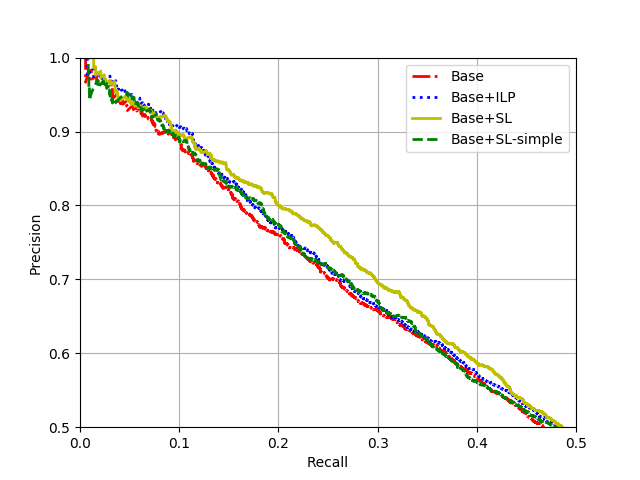
\includegraphics[width=8cm]{./result-figure/DBpedia-CNN-result.png}
		\caption{The DBpedia Dataset}
		\label{fig:dbpedia}
	\end{minipage}
	\begin{minipage}[t]{0.48\textwidth}
		\centering
		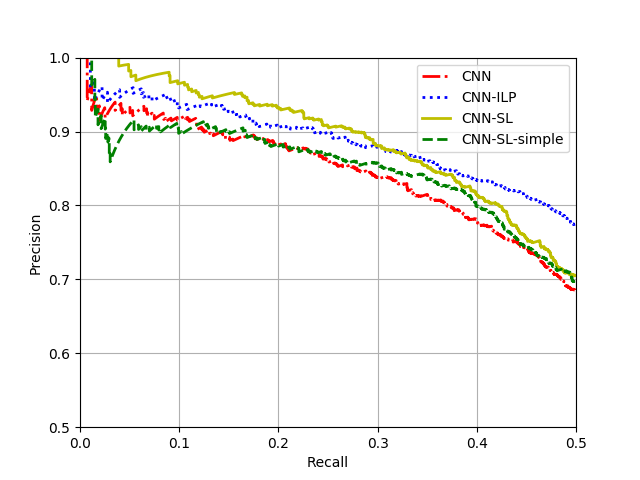
\includegraphics[width=8cm]{./result-figure/Chinese-CNN-result.png}
		\caption{The Chinese Dataset}
		\label{fig:chinese}
	\end{minipage}
\end{figure}

\paragraph{Compare with Base Model}
%Compare the semantic loss method and the base model (clear improvement).
Figure ~\ref{fig:dbpedia} and Figure ~\ref{fig:chinese} shows that compared with the baseline, our framework performs consistently better in the DBpedia dataset and Chinese dataset. 
%In order to father demonstrate the semantic loss term helps to encode the constraints into relation extraction model, we count the tuple pairs that violates relation constraints introduced in Sec.~\ref{sec:constraints}, the results is show in Table ~\ref{table:violate-count}.
%IPE:  473.0 WPC:  440.0 CPNI:  273.0 CNN_C:  2123.0 SL_C:  2209.0

In order to study how our framework improves the performances on the DBpedia dataset and the Chinese dataset, we further dig into the predictions of Base Model and SL Model, we find that our SL model corrects the Base Model's predictions to satisfy the constraints. Take \textless Center For Responsible Lending, North Carolina\textgreater and \textless Meredith College, North Carolina \textgreater as an example. The Base Model predicts relations $Location$ and $CoachedTeam$ for them, and our SL Model predicts $Location$ and $State$. We could find that $Location$ should has a place as its subject, and $ CoachedTeam $'s subject type should be Team, so there exists a conflict between the two predictions, and our SL Model eliminates the conflict through automatically learning constrain knowledge when training. 
%28 8 28 45 
\iffalse
\begin{table}
	\centering  
	\scriptsize  
	\caption{violate count}  
	\begin{tabular}{|c|c|c|c|c|}  
		\hline  
		 &Model&Type Violates&Cardinality Violates&Total\\  
		\hline 
		\multirow{2}*{DBpedia} & CNN & - & - & -\\
		~ & CNN-SL & - & - & -\\
		\hline 
		\multirow{2}*{Chinese} & CNN & - & - & -\\
		~ & CNN-SL & - & - & -\\ 
		\hline   
	\end{tabular} 
	
	\label{table:violate-count}  
\end{table}
\fi
\iffalse
\begin{figure}
	\centering
	\includegraphics[width=.4\textwidth]{./result-figure/CNN0-1.png}
	\caption{The DBpedia Dataset}
\end{figure}
\fi


\paragraph{Compare with ILP Method}
%Compare the semantic loss method and ILP.
%NOTE: clw also use cardinality constraints
We use the same constraints information as the \ILP method of \cite{chen2014encoding}, and Figure ~\ref{fig:dbpedia} and Figure ~\ref{fig:chinese} shows that our SL method delivers superior performance compared to \ILP method in both DBpedia dataset and Chinese dataset.

For DBpedia dataset, our method's performance is over \ILP method almost on all precision point. We think this is mainly because \ILP is a post-processing method which choose the most possible prediction that satisfy the constraints from the top three candidate results for every entity pairs, and this would drop some high score predictions, so for the high precision point, our SL method have better performance for both DBpedia dataset and Chinese Dataset. We also find that when recall in (0.3, 0.5), the \ILP is better than our SL method for Chinese Dataset, we think this is because adding constraints for Chinese dataset is much better than DBpedia dataset, the \ILP would drop more high score predictions and the right prediction corrected by \ILP is more likely appear at recall range (0.3, 0.5).

As we all know, the performance of high precision in PR curve is more important that the low precision, so totally our SL model gets superior performance than \ILP.
\paragraph{Compare with Simplified Semantic Loss}
%Compare the semantic loss method and the simplified semantic loss.
%Both on PR-curve, and on time.
To reduce the time cost brought by semantic loss, we simplify the calculating of semantic loss by choosing some constraints from C in ~\ref{seq:semantic_loss} as new $\bm{C'}$, the $ \bm{C'} $ includes one most related constraint with the gold information of tuple pairs and 5 random sampling constraints, then we get the simplified semantic loss $ L^{s}_{simple}(\bm{C'}, \bm{p}) $ as follows:

\begin{equation}
\label{seq:semantic_loss_simple}
L^{s}_{simple}(\bm{C'}, \bm{p}) = -log\sum\limits_{\bm x\models\bm{C'}}\prod\limits_{i:\bm x\models X_i}p_i\prod\limits_{i:\bm x\models \neg X_i}(1-p_i)
\end{equation}

This simplified semantic loss will significantly reduce the extra time overhead compared with original semantic loss, 7 times in DBpedia dataset, 3 times in Chinese dataset(because the constraints over Chinese is less than DBpedia). And both in DBpedia dataset and Chinese dataset the simplified semantic loss have improvement over Base Model, especially in DBpedia, it has comparable result with \ILP.


